\documentclass[conference]{IEEEtran}
\usepackage{cite}
\usepackage{amsmath,amssymb,amsfonts}
\usepackage{algorithmic}
\usepackage{graphicx}
\usepackage{textcomp}
\usepackage{xcolor}
\graphicspath{{sources/}}
\def\BibTeX{{\rm B\kern-.05em{\sc i\kern-.025em b}\kern-.08em
    T\kern-.1667em\lower.7ex\hbox{E}\kern-.125emX}}
\begin{document}

\title{Noobcash\\
}

\author{\IEEEauthorblockN{Georgios Kyriakopoulos}
\IEEEauthorblockA{\textit{School of ECE, NTUA} \\
\textit{Department of Computer Science}\\
Athens, Greece \\
el18153@mail.ntua.gr }
\and
\IEEEauthorblockN{Eleni Tsertou}
\IEEEauthorblockA{\textit{School of ECE, NTUA} \\
\textit{Department of Computer Science}\\
Athens, Greece \\
el18165@mail.ntua.gr}
\and
\IEEEauthorblockN{Serafeim Tzelepis}
\IEEEauthorblockA{\textit{School of ECE, NTUA} \\
\textit{Department of Computer Science}\\
Athens, Greece \\
el18849@mail.ntua.gr}
}

\maketitle

\begin{abstract}
The Noobcash project is a blockchain system designed to facilitate secure and decentralized transactions without the need for a central authority, implemented in Python \cite{b1}. The system achieves this by utilizing a distributed database, which ensures that all nodes within the network have access to the same information and can verify the validity of any transaction. As part of the project's development, several experiments were conducted to analyze the system's performance in terms of throughput and block times under varying conditions. These experiments involved testing different combinations of block capacity and mining difficulty. Additionally, the scalability of the system was tested by increasing the number of nodes within the network from 5 to 10. Through these experiments, valuable insights were gained into the system's behavior under different conditions, which can inform future improvements and developments in blockchain technology.
\end{abstract}

\begin{IEEEkeywords}
blockchain, cryptocurrency, python, experiments, proof-of-work, throughput, block time, block capacity, mining difficulty, scalability.
\end{IEEEkeywords}

\section{\textbf{Introduction}}
Blockchain technology has become increasingly popular in recent years due to its ability to facilitate secure and decentralized transactions without the need for a central authority. One of the most well-known applications of blockchain technology is in the realm of cryptocurrencies, which rely on blockchain systems to enable users to transact with each other securely and efficiently. 

The Noobcash project is a python-based implementation of a blockchain system that aims to provide a basic but functional example of a blockchain system. The system uses Proof-of-Work to ensure consensus between nodes, and it is designed to enable secure and decentralized transactions between users without the need for a central authority. Thorough explanation about the implementation of the system and how it works are provided in an upcoming section.

As part of the project's development, a series of experiments were conducted to analyze the system's performance under different conditions. These experiments included testing different combinations of block capacity and mining difficulty to determine the system's throughput and block times. Additionally, the scalability of the system was tested by increasing the number of nodes within the network from 5 to 10.

This paper is backed by a GitHub repository \cite{b2} \cite{b3}, which contains the source code of the system, the scripts used for installation and testing, as well as analytics for the results.

\section{\textbf{Setup}}
In this section, we outline a brief explanation of the setup that was utilized to run the blockchain and the experiments.

We used the okeanos IAAS \cite{b4}, which is GRNET's cloud service, for the Greek Research and Academic Community, to acquire 5 virtual machines for our study. Each machine has the same following specifications:

\begin{itemize}
\item CPU: 2 Cores - Intel\textregistered\ Xeon\textregistered\ CPU E5-2650 v3
\item RAM: 2GB
\item Disk: 30GB
\item Operating System: Ubuntu Server 16.04.3 LTS
\end{itemize}

Those 5 machines were used to set up a 5-node cluster. We also set up a local network (192.168.2.0/24) so that the 5 nodes could communicate with each other. After setting up our machines, we used SSH in order to connect and have access to them and proceed with the configuration.

We then installed Python3.8 \cite{b1} by building it from source and pip \cite{b5} using a script for all nodes. At that point, we were ready to proceed with the implementation of our blockchain system in Python.

\section{\textbf{Implementation}}
We developed our blockchain source code by dividing it into several Python classes. The classes we used are:

\begin{itemize}
\item \textbf{Block}
\item \textbf{Blockchain}
\item \textbf{Node}
\item \textbf{Transaction}
\item \textbf{TransactionInput}
\item \textbf{TransactionOutput}
\item \textbf{Wallet}
\end{itemize}

On the following subsections, we will analyse each class separately.

\subsection{Block}
This class has the following instance variables:

\begin{itemize}
\item \textbf{index}: index of the Block
\item \textbf{timestamp}: timestamp of the Block's creation
\item \textbf{transactions}: list of the Block's transactions
\item \textbf{nonce}: proof-of-work
\item \textbf{previous\_hash}: hash of the previous Block
\item \textbf{hash}: hash of the Block
\end{itemize}

The following instance methods were also developed:

\begin{itemize}
\item \textbf{add\_transaction\_and\_check}: adds a new transaction in the Block and checks if the Block has reached its capacity
\item \textbf{hash\_block}: calculates the hash of the Block
\end{itemize}

\subsection{Blockchain}
This class has the following instance variables:

\begin{itemize}
\item \textbf{blocks}: list of validated blocks in the chain
\end{itemize}

This class has no instance methods.

\subsection{Node}
This class has the following instance variables:

\begin{itemize}
\item \textbf{id}: id of the node
\item \textbf{chain}: blockchain of the node
\item \textbf{wallet}: wallet of the node
\item \textbf{ring}: information about others (id, ip, port, public\_key, balance)

\item \textbf{filter\_lock}: lock in order to provide mutual exclusion while filtering blocks
\item \textbf{chain\_lock}: lock in order to provide mutual exclusion while updating the chain
\item \textbf{block\_lock}: lock in order to provide mutual exclusion while updating blocks
    
\item \textbf{unconfirmed\_blocks}: queue that contains all the blocks waiting to be mined
\item \textbf{current\_block}: the block that the node currently fills with transactions
\item \textbf{capacity}: max number of transactions in each block
\item \textbf{stop\_mining}: flag to stop mining when a confirmed block arrives
\end{itemize}

The following instance methods were also developed:

\begin{itemize}
\item \textbf{create\_new\_block}: creates a new block
\item \textbf{register\_node\_to\_ring}: registers a new node in the ring, called only by the bootstrap node
\item \textbf{create\_transaction}: creates a new transaction, after gathering the inputs from the utxos
\item \textbf{add\_transaction\_to\_block}: adds a transaction to a block, check if mining is needed and update the wallet and balances of participating nodes
\item \textbf{broadcast\_transaction}: broadcasts a transaction to the network, utilizing threads
\item \textbf{validate\_transaction}: validates an incoming transaction, by checking the signature, the inputs and the outputs
\item \textbf{mine\_block}: implements the proof-of-work algorithm
\item \textbf{broadcast\_block}: broadcasts a transaction to the network, utilizing threads
\item \textbf{validate\_previous\_hash}: validates the previous hash of an incoming block
\item \textbf{validate\_block}: validates a block, by validating its hash and its previous hash
\item \textbf{filter\_blocks}: filters the queue of the unconfirmed blocks, by removing the transactions that are included in a mined block
\item \textbf{share\_ring}: shares your ring to a specified node
\item \textbf{validate\_chain}: validates all the blocks of a chain
\item \textbf{share\_chain}: shares your blockchain to a specified node
\item \textbf{resolve\_conflicts}: resolves conflicts of multiple blockchains, by keeping the longest chain when a new block that can't be validated is received
\end{itemize}

\subsection{Transaction}
This class has the following instance variables:

\begin{itemize}
\item \textbf{sender}: sender's public key
\item \textbf{sender\_id}: id of the sender
\item \textbf{receiver}: receiver's public key
\item \textbf{receiver\_id}: id of the receiver
\item \textbf{amount}: amount of nbc to transfer
\item \textbf{total}: total amount that sender sends
\item \textbf{inputs}: list of TransactionInput
\item \textbf{id}: hash of the transaction
\item \textbf{outputs}: list of TransactionOutput
\item \textbf{signature}: signature of the transaction
\end{itemize}

The following instance methods were also developed:

\begin{itemize}
\item \textbf{convert\_to\_list}: list representation of a Transaction
\item \textbf{hash\_transaction}: calculates the hash of the Transaction
\item \textbf{calculate\_outputs}: computes Transaction outputs
\item \textbf{sign\_transaction}: signs the Transaction using a private key
\item \textbf{verify\_signature}: verifies the signature of a Transaction
\end{itemize}

\subsection{TransactionInput}
This class has the following instance variables:

\begin{itemize}
\item \textbf{output\_id}: id of the TransactionOutput that is used as TransactionInput
\end{itemize}

This class has no instance methods.

\subsection{TransactionOutput}
This class has the following instance variables:

\begin{itemize}
\item \textbf{transaction\_id}: id of the transaction
\item \textbf{target}: target of the TransactionOutput
\item \textbf{amount}: amount of nbc to be credited to the target
\item \textbf{unspent}: boolean of whether this output has been used or not
\end{itemize}

This class has no instance methods.

\subsection{Wallet}
This class has the following instance variables:

\begin{itemize}
\item \textbf{private\_key}: private key of the node
\item \textbf{public\_key}: public key of the node, also its address
\item \textbf{transactions}: list that contains the transactions of the wallet
\end{itemize}

The following instance methods were also developed:

\begin{itemize}
\item \textbf{wallet\_balance}: calculates balance of the wallet based on the utxos
\end{itemize}

\section{\textbf{REST API and Client}}

Now, after introducing the classes and methods implemented for the blockchain, it is important to highlight the parts that bring the system to life. These include the endpoints we developed for the REST API, a simple client in the form of a CLI (command-line interface) and a script to test some sample transactions.

\subsection{Endpoints}
The REST API we developed utilizes the endpoints below:

\begin{itemize}
\item \textbf{register\_node}: registers a new node in the network, called only by the bootstrap node
\item \textbf{validate\_transaction}: validates an incoming transaction
\item \textbf{receive\_transaction}: receives a transaction and adds it to a block
\item \textbf{receive\_block}: receives a block, validates it and adds it to the blockchain
\item \textbf{receive\_ring}: receives the ring from bootstrap
\item \textbf{receive\_chain}: receives the blockchain
\item \textbf{send\_chain}: sends your chain to another node
\item \textbf{create\_transaction}: creates a new transaction
\item \textbf{get\_balance}: gets balance of the node
\item \textbf{get\_transactions}: gets transactions of the last confirmed block
\item \textbf{get\_id}: gets id of the node
\item \textbf{get\_metrics}: gets metrics of the network
\end{itemize}

\subsection{Noobcash Client}
To develop a client for our blockchain, we opted for a simple CLI client, using the PyInquirer module \cite{b6}.
The client has the following commands available:

\begin{itemize}
\item \textbf{new transaction}: create a new transaction, specifying the amount of NBC coins to send and the receiver's id
\item \textbf{view last transactions}: print the transactions contained in the last validated block of the Noobcash blockchain
\item \textbf{balance}: print the balance of the wallet
\item \textbf{help}: explanation of the above commands
\end{itemize}

\subsection{How to Run and Test}
We have also implemented a \verb|main.py| file that starts the REST API on the node and then, based on the command line arguments used when running it, initializes a node.

More specifically, when running the \verb|main.py| file, the following arguments can be defined:

\begin{itemize}
\item \textbf{-p} \verb|<port>|: port to listen on
\item \textbf{-n} \verb|<number-of-nodes>|: number of nodes in the blockchain
\item \textbf{-c} \verb|<capacity>|: capacity of a block
\item \textbf{-b}: flag that is set if current node is the bootstrap
\end{itemize}

The first 3 arguments are required for every node, while the last one should only be set on the bootstrap node (the first one on the network).

In the case of the bootstrap node, it registers itself on the ring, creates the genesis block and the first transaction, adds it in the genesis block and then waits for other nodes to join. When another node initializes, it sends a request to the bootstrap node to be registered on the ring. When all nodes have joined, the bootstrap node broadcasts the ring, the blockchain up to that point and also sends each node 100 NBC coins.

Bear in mind that in the case of a network with 5 nodes, each machine needs to run the REST API once, using the \verb|main.py| file on a port of choice (default 5000). However, if the number of nodes is 10, then each machine needs to run the REST API twice, on two different ports (e.g. 5000 and 6000). These 2 different ports are used to distinguish between the two nodes that need to run on the same machine.

Then, the noobcash client (CLI) can be used to interact with the blockchain (creating transactions, checking the balance etc), or a script that runs a few sample transactions may be executed, to test the system. 

The client can be run by executing the \verb|noobcash.py| file, specifying the \textbf{-p} \verb|<port>| argument, which is the port that the REST API is listening on that node. The client will then ask the user to input a command, which can be one of the above mentioned commands.

The test script can be used on any node by executing the \verb|run_test_files.py| file and will run 100 transactions sending NBC coins to other nodes. It requires a \textbf{-d} \verb|<directory>| command line argument, specifying the path to the directory of the transactions and a \textbf{-p} \verb|<port>|, specifying the port that the REST API is listening on that node.

\section{\textbf{Experiments}}
\subsection{Metrics}
We ran some experiments on our blockchain, testing different combinations of block capacity and mining difficulty. These tests were conducted to measure the system's performance using two metrics, throughput and block times. We also tested the scalability of our system, by running the blockchain with 5 and 10 nodes in the network.

\subsection{Graphs}
The results of the above tests can be summarized in the following graphs. The first graph is comparing the throughput for 5 and 10 nodes based on the different configurations of block capacity and mining difficulty. The second graph is doing the same but for block time. The next two graphs provide a clearer view of how the scaling of the system's number of nodes affects the throughput and block time.

\begin{figure}[htbp]
\centerline{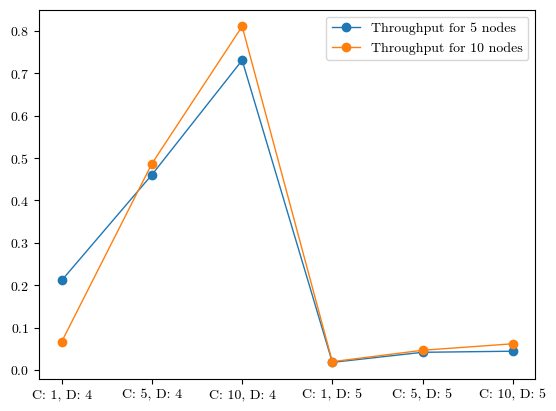
\includegraphics[width=0.5\textwidth]{throughput-capacity-difficulty.png}}
\caption{Throughput relative to Capacity (C) and Difficulty (D)}
\label{throughput-cd}
\end{figure}

\begin{figure}[htbp]
\centerline{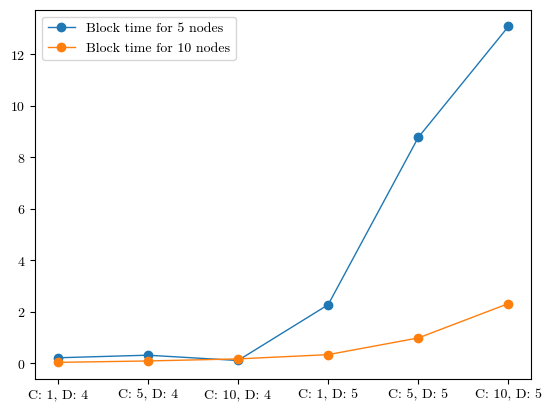
\includegraphics[width=0.5\textwidth]{block-time-capacity-difficulty.png}}
\caption{Block time relative to Capacity (C) and Difficulty (D)}
\label{blocktime-cd}
\end{figure}

\begin{figure}[htbp]
\centerline{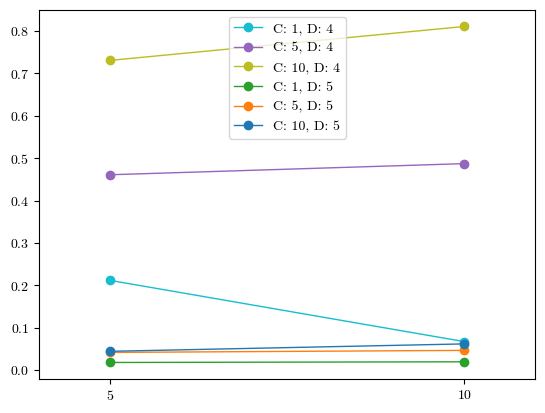
\includegraphics[width=0.5\textwidth]{throughput-number-of-nodes.png}}
\caption{Throughput relative to Number of Nodes}
\label{throughput-non}
\end{figure}

\begin{figure}[htbp]
\centerline{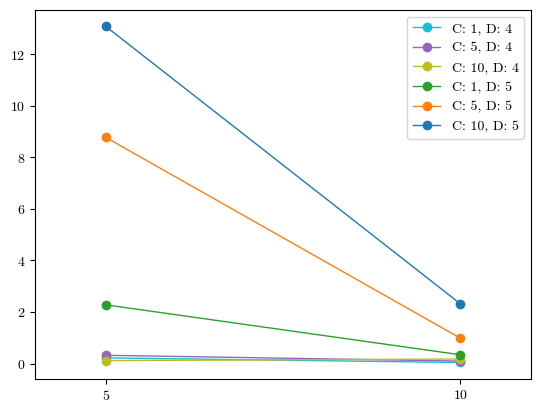
\includegraphics[width=0.5\textwidth]{block-time-number-of-nodes.png}}
\caption{Block time relative to Number of Nodes}
\label{blocktime-non}
\end{figure}

\subsection{Comments}
Based on Figure \ref{throughput-cd}, we can see that the throughput of the system increases as the block capacity increases, since less time is spend mining, because more transactions can fit into one block and mining is needed less frequently. As difficulty increases, the throughput decreases, since mining is now harder and requires more time to finish.

About Figure \ref{blocktime-cd}, it is clear that as difficulty increases, the block time will increase as well, considering that mining is harder and will certainly take up more time on average to find the right nonce and hash. Block time also increases as capacity increases, since now the block contains more transactions and all the operations on it, including calculating the hash, are expected to take up more time.

For Figure \ref{throughput-non}, in most configurations there is a small but noticeable increase in the system throughput from 5 to 10 nodes. When increasing the number of nodes, there are more miners available to help speed up the mining process and therefore increase the throughput of the system. However, with more nodes, there are also more blocks created and there is added network latency and communication overhead. So, an increase is possible and expected, but not to a great extent.

Finally, on Figure \ref{blocktime-non}, block time is significantly reduced. That is more noticeable on the configurations with higher mining difficulty. This behavior is expected, when considering that there are more miners available to mine every block, which will lead to lower block time.

\subsection{Conclusion}

Based on the experiments conducted on the blockchain system, it is evident that the block capacity and mining difficulty have a significant impact on the system's throughput and block time. Increasing the block capacity can increase the throughput, while increasing the mining difficulty can decrease the throughput and increase the block time. Additionally, increasing the number of nodes in the network can slightly increase the throughput, but will also heavily reduce the block time, more so when the mining difficulty is higher.

Overall, these experiments highlight the importance of carefully optimizing the block capacity, mining difficulty, and network infrastructure to achieve optimal performance in a blockchain system.

\begin{thebibliography}{00}
\bibitem{b1} “Welcome to Python.org,” Python.org. [Online]. Available: https://www.python.org/.
\bibitem{b2} G. Kyriakopoulos, E. Tsertou, S. Tzelepis, “geokyr/ntua-distributed-systems: Simple blockchain system project in Python, that records transactions between participants and ensures consensus using Proof-of-Work for the Distributed Systems course at ECE NTUA,” GitHub. [Online]. Available: https://github.com/geokyr/ntua-distributed-systems.
\bibitem{b3} S. Tzelepis, “SerTze/ntua-distributed-systems: Blockchain project in Python. Noobcash is a simple blockchain system that records transactions between participants and ensures consensus using Proof-of-Work,” GitHub. [Online]. Available: https://github.com/SerTze/ntua-distributed-systems.
\bibitem{b4} “~Okeanos,” ~okeanos Dashboard. [Online]. Available: https://accounts.okeanos.grnet.gr/.
\bibitem{b5} “Pip,” PyPI. [Online]. Available: https://pypi.org/project/pip/.
\bibitem{b6} “Pyinquirer,” PyPI. [Online]. Available: https://pypi.org/project/PyInquirer/.
\end{thebibliography}

\end{document}
